% Als je labels toe wilt voegen, doe het dan consequent
% voor een section ---> \label{sec:name_of_block}
%voor een subsection ---> \label{ssec:name_of_subsec}
%voor een subsubsec --> \label{sssec:name_of_subsubsec} en zo door

%Template voor elk apart blok EPO3 A4
\documentclass{scrartcl} % scrartcl of scrreprt
% Include all project wide packages here.
\usepackage{fullpage}
\usepackage{polyglossia}
\setmainlanguage{dutch}
\usepackage{csquotes}
\usepackage{graphicx}
\usepackage{epstopdf}
\usepackage{pdfpages}
\usepackage{caption}
\usepackage[list=true]{subcaption}
\usepackage{float}
%\usepackage{mathtools}
\usepackage{standalone}
\usepackage{import}
\usepackage{tocloft}
\usepackage{wrapfig}
\usepackage{authblk}
\usepackage{array}
\usepackage{booktabs}
\usepackage[toc,page,title,titletoc]{appendix}
\usepackage{xunicode}
\usepackage{amsmath}
\usepackage{fontspec}
\usepackage{unicode-math}
\usepackage[
    backend=bibtexu,
	texencoding=utf8,
bibencoding=utf8,
    style=ieee,
    sortlocale=nl_NL,
    language=auto
]{biblatex}
\usepackage{listings}
\newcommand{\includecode}[3][c]{\lstinputlisting[caption=#2, escapechar=, style=#1]{#3}}
\newcommand{\superscript}[1]{\ensuremath{^{\textrm{#1}}}}
\newcommand{\subscript}[1]{\ensuremath{_{\textrm{#1}}}}


\newcommand{\chapternumber}{\thechapter}
\renewcommand{\appendixname}{Bijlage}
\renewcommand{\appendixtocname}{Bijlagen}
\renewcommand{\appendixpagename}{Bijlagen}

\usepackage[hidelinks]{hyperref} %<--------ALTIJD ALS LAATSTE
 
\renewcommand{\familydefault}{\sfdefault}

\setmainfont[Ligatures=TeX]{Myriad Pro}
\setmathfont{Asana Math}
\setmonofont{Lucida Console}

\usepackage{titlesec, blindtext, color}
\definecolor{gray75}{gray}{0.75}
\newcommand{\hsp}{\hspace{20pt}}
\titleformat{\chapter}[hang]{\Huge\bfseries}{\chapternumber\hsp\textcolor{gray75}{|}\hsp}{0pt}{\Huge\bfseries}
\renewcommand{\familydefault}{\sfdefault}
\renewcommand{\arraystretch}{1.2}
\setlength\parindent{0pt}

%For code listings
\definecolor{black}{rgb}{0,0,0}
\definecolor{browntags}{rgb}{0.65,0.1,0.1}
\definecolor{bluestrings}{rgb}{0,0,1}
\definecolor{graycomments}{rgb}{0.4,0.4,0.4}
\definecolor{redkeywords}{rgb}{1,0,0}
\definecolor{bluekeywords}{rgb}{0.13,0.13,0.8}
\definecolor{greencomments}{rgb}{0,0.5,0}
\definecolor{redstrings}{rgb}{0.9,0,0}
\definecolor{purpleidentifiers}{rgb}{0.01,0,0.01}


\lstdefinestyle{csharp}{
language=[Sharp]C,
showspaces=false,
showtabs=false,
breaklines=true,
showstringspaces=false,
breakatwhitespace=true,
escapeinside={(*@}{@*)},
columns=fullflexible,
commentstyle=\color{greencomments},
keywordstyle=\color{bluekeywords}\bfseries,
stringstyle=\color{redstrings},
identifierstyle=\color{purpleidentifiers},
basicstyle=\ttfamily\small}

\lstdefinestyle{c}{
language=C,
showspaces=false,
showtabs=false,
breaklines=true,
showstringspaces=false,
breakatwhitespace=true,
escapeinside={(*@}{@*)},
columns=fullflexible,
commentstyle=\color{greencomments},
keywordstyle=\color{bluekeywords}\bfseries,
stringstyle=\color{bluestrings},
identifierstyle=\color{purpleidentifiers}
}

\lstdefinestyle{vhdl}{
language=VHDL,
showspaces=false,
showtabs=false,
breaklines=true,
showstringspaces=false,
breakatwhitespace=true,
escapeinside={(*@}{@*)},
columns=fullflexible,
commentstyle=\color{greencomments},
keywordstyle=\color{bluekeywords}\bfseries,
stringstyle=\color{redstrings},
identifierstyle=\color{purpleidentifiers}
}

\lstdefinestyle{xaml}{
language=XML,
showspaces=false,
showtabs=false,
breaklines=true,
showstringspaces=false,
breakatwhitespace=true,
escapeinside={(*@}{@*)},
columns=fullflexible,
commentstyle=\color{greencomments},
keywordstyle=\color{redkeywords},
stringstyle=\color{bluestrings},
tagstyle=\color{browntags},
morestring=[b]",
  morecomment=[s]{<?}{?>},
  morekeywords={xmlns,version,typex:AsyncRecords,x:Arguments,x:Boolean,x:Byte,x:Char,x:Class,x:ClassAttributes,x:ClassModifier,x:Code,x:ConnectionId,x:Decimal,x:Double,x:FactoryMethod,x:FieldModifier,x:Int16,x:Int32,x:Int64,x:Key,x:Members,x:Name,x:Object,x:Property,x:Shared,x:Single,x:String,x:Subclass,x:SynchronousMode,x:TimeSpan,x:TypeArguments,x:Uid,x:Uri,x:XData,Grid.Column,Grid.ColumnSpan,Click,ClipToBounds,Content,DropDownOpened,FontSize,Foreground,Header,Height,HorizontalAlignment,HorizontalContentAlignment,IsCancel,IsDefault,IsEnabled,IsSelected,Margin,MinHeight,MinWidth,Padding,SnapsToDevicePixels,Target,TextWrapping,Title,VerticalAlignment,VerticalContentAlignment,Width,WindowStartupLocation,Binding,Mode,OneWay,xmlns:x}
}

%defaults
\lstset{
basicstyle=\ttfamily\small,
extendedchars=false,
numbers=left,
numberstyle=\ttfamily\tiny,
stepnumber=1,
tabsize=4,
numbersep=5pt
}


\author{Efraïm Eland}% <------fill in your name
\title{EPO3: Eindrapport - Draw-pixel}

\begin{document}
\section{Draw-rect} %<----- fill in section name
\label{sec:draw-rect}  %<-----fill in lable name

\newcommand{\tss}{\textsubscript}

%specs
\subsection{Specificaties}
De module draw\_rect is een module die, wanneer hij toegang heeft tot het RAM (draw\_can\_acces = '1'), de coördinaten van een vierkant met de gewenste kleur (color), synchroon met de klok wegschrijft naar het VRAM. Hierbij moet de module alle coördinaten die hij nodig heeft, om het vierkant af te beelden, bepalen aan de hand van de aan de input aangeboden linkerboven coördinaat (x\tss{0},y\tss{0}) en rechteronder coördinaat (x\tss{1},y\tss{1}). Daarnaast moet de module ook nog een onderscheid maken tussen het niet opvullen van het vierkant (enable = '1') en het wel opvullen van het vierkant (enablef = '1'). Het wegschrijven van coördinaten moet in de niet-actieve screenbuffer (not asb) worden gedaan, zodat het vierkant na de volgende schermbufferwisseling door de VGA-controller op het scherm wordt getekend.
\\\\
Als laatste is het handig dat de module aangeeft dat hij bezig is met het wegschrijven van coördinaten naar het VRAM (draw\_write = '1') en is het handig als hij een signaal afgeeft wanneer hij klaar is (done = '1').
\\\\
Een overzicht van alle aansluitingen van de module zijn te vinden in figuur \ref{fig:draw_rect}.

\begin{figure}[H]
	\centering
	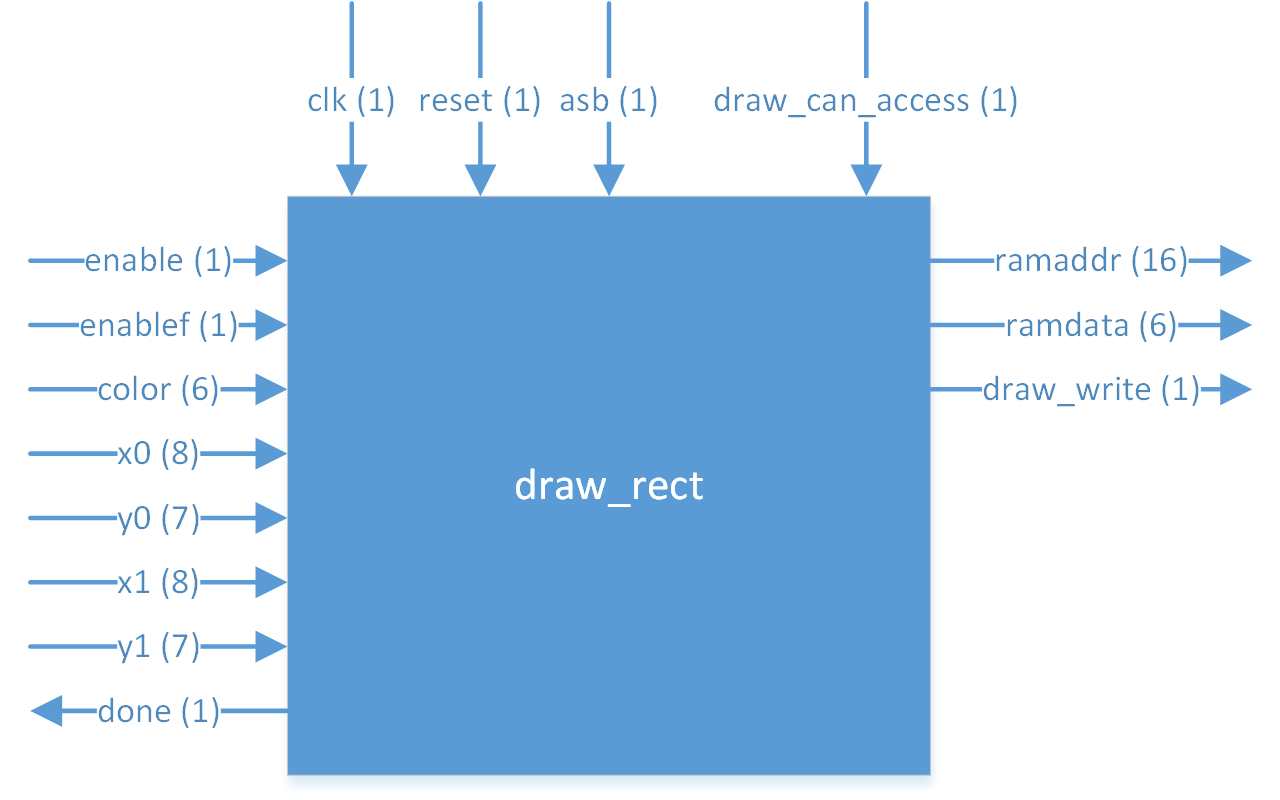
\includegraphics[width=\textwidth]{resources/draw_rect.png}
	\caption{Schematisch overzicht van de draw\_rect module}
	\label{fig:draw_rect}
\end{figure}

%Ontwerp en implementatie
\subsection{Ontwerp en implementatie}
In bijlage \ref{appsec:draw_rect.vhdl} is de VHDL entity van draw-rect te zien en in bijlage \ref{appsec:draw_rect-behaviour.vhdl} is de bijbehorende VHDL behaviour te zien. Zodra het ingangssignaal draw\_can\_access hoog is, is de RAM vrij om beschreven te worden en begint de module rechtsonderin met tekenen op coördinaat (x\tss{1},y\tss{1}). De module zet op de actieve klokflank de huidige coördinaat op het uitgangssignaal ramaddr (samen met het not asb signaal) en zet de kleur op het uitgangssignaal ramdata. Ook wordt er aan de RAM controller doorgegeven dat de module de data van ramaddr en ramdata op het RAM wilt schrijven door middel van het signaal draw\_write = '1'.
\\\\
Vervolgens gaat de module een stap naar links maken en bevindt zich dan op het punt (x\tss{1} -1, y\tss{1}). Deze stapjes worden net zolang herhaald, totdat de x-coördinaat het punt x0 heeft bereikt. Daarna wordt er een sprong terug gemaakt, één positie boven het punt waar de module is begonnen met tekenen, namelijk (x\tss{1}, y\tss{1} -1). Vervolgens herhaalt het proces zich tot het punt (x\tss{0}, y\tss{0}) is bereikt. Afhankelijk van het ingangssignalen enable en enablef kan de rechthoek al dan niet worden ingekleurd.
\\\\
Nadat de module klaar is met het bepalen van de coördinaten van de rechthoek, wordt het uitgangssignaal done = '1'.

%VHDL simulatie
\subsection{VHDL simulatie}
Voor het testen van de VHDL code is een testbench geschreven en gesimuleerd in ModelSim. De behaviour van deze testbench is te vinden in bijlage \ref{appsec:draw_rect_tb-behaviour.vhdl}. Aan de ingang worden o.a. twee coördinaten doorgegeven en een kleurcode. Enable en enablef werden gebruikt om aan te geven dat de rechthoek niet ingekleurd moest worden.
\\\\
De simulatie werkte goed. Op de uitgangen ramdata en ramaddr kwamen de juiste signalen te staan. Nadat de module klaar was, kwam er een signaal done = '1' op de uitgang te staan. Ook waren de signalen synchroon met de clock. De volgende stap is het synthetiseren van de VHDL code. In figuur \ref{fig:draw_rect-vhdlsim} is een fragment van deze simulatie te zien in ModelSim.
\\\\

\begin{figure}[H]
	\centering
	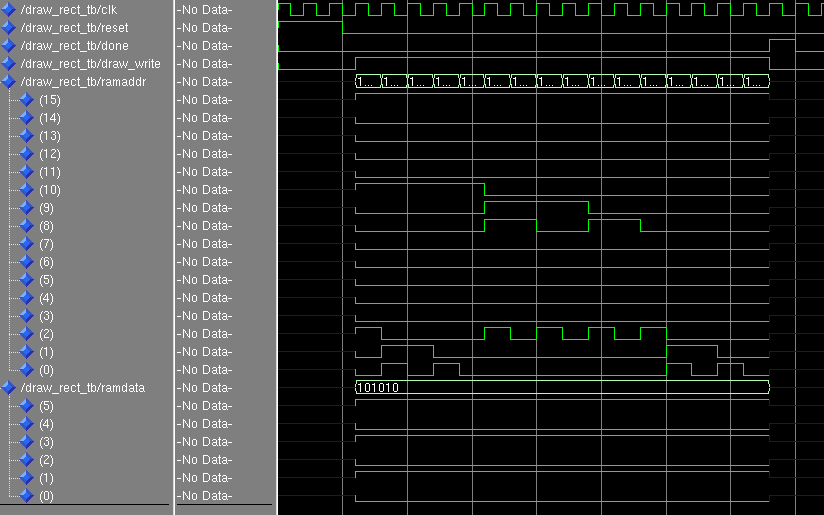
\includegraphics[width=\textwidth]{resources/draw_rect-vhdlsim.png}
	\caption{Een fragment uit de waveform van de draw\_rect testbench}
	\label{fig:draw_rect-vhdlsim}
\end{figure}

%Synthese
\subsection{Synthese en lay-out}
Het synthetiseren van de draw\_rect module verliep over het algemeen soepel. M.b.v. de Place \& route functie van het programma Seadali konden niet alle verbindingen worden gemaakt. Dit probleem is verholpen door handmatig met de row placer functie rijen op te schuiven en vervolgens Seadali laten routen met de trout functie. Hierbij kwam het programma op een totaal van 4728 transistoren, waarvan er 2383 daadwerkelijk werden gebruikt. De efficiëntie voor deze module bedraagt dus 50.40\%.

%Switchlevel test
\subsection{Switch-level simulatie}
De gesynthetiseerde schakeling is gesimuleerd met SLS. Deze simulatie is vervolgens vergeleken met de VHDL simulatie die in ModelSim plaats heeft gevonden. Deze vergelijking leverde geen bijzonderheden op. Ook is de lay-out gesimuleerd met SLS en vergeleken met de VHDL simulatie. En ook hier traden geen bijzonderheden op.

%Conclusie
\subsection{Conclusie}
Aan de hand van de simulaties van de VHDL code, gesynthetiseerde schakeling en de lay-out kan geconcludeerd worden dat draw\_rect op alle gebieden voldoet aan de specificaties. De efficiëntie van de lay-out zou eventueel nog verhoogd kunnen worden als de VHDL code zou veranderen of de gesynthetiseerde schakeling beter geoptimaliseerd zou worden. Al met al is de module draw\_rect met een lay-out efficiëntie van 50.40\% een succes!

\end{document}
